\begin{figure}[H]
  \centering
  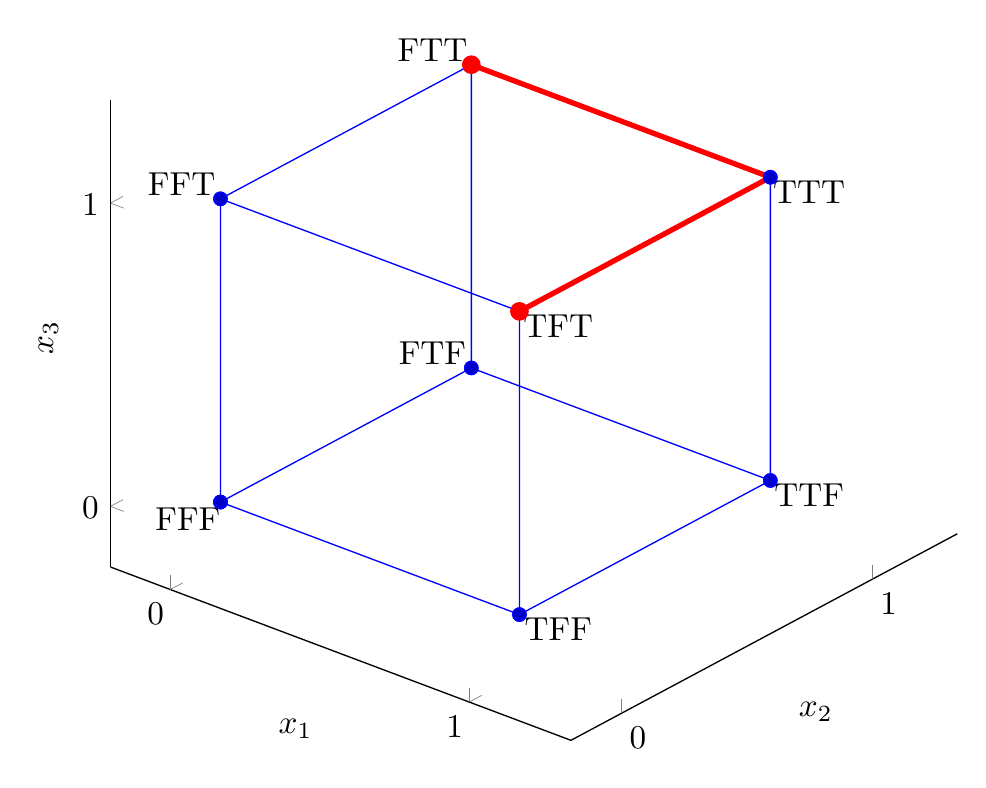
\begin{tikzpicture}[scale=1.2, x={({1}, {0})}]
    \begin{axis}[
      view/h=40,
      width=300pt,
      height=300pt,
      axis lines*=left,
      xmin=-0.2,xmax=1.2,
      ymin=-0.2,ymax=1.2,
      zmin=-0.2,zmax=1.2,
      enlargelimits=upper,
      xtick={0,1},
      ytick={0,1},
      ztick={0,1},
      xlabel={$x_1$},
      ylabel={$x_2$},
      zlabel={$x_3$}
    ]
      % pre-cube
      \addplot3 coordinates {(0,0,0) (0,1,0) (0,1,1) (0,0,1) (0,0,0)
        (0,0,1) (1,0,1) (1,0,0) (0,0,0) (1, 0, 0) (1,1,0) (0,1,0) (0,1,1) (1,1,1) (1,1,0) (1,1,1) (1,0,1)};

      \addplot3 [only marks, mark=*, fill=red, draw=red, ultra thick] coordinates {(0,1,1) (1,0,1)};

      \node (A) at (axis cs:0,-0.13,0) {FFF};
      \node (B) at (axis cs:-0.13,1,0) {FTF};
      \node (C) at (axis cs:-0.13,1,1) {FTT};
      \node (D) at (axis cs:-0.13,0,1) {FFT};
      \node (E) at (axis cs:1.13,0,1) {TFT};
      \node (F) at (axis cs:1.13,0,0) {TFF};
      \node (G) at (axis cs:1.13,1,0) {TTF};
      \node (H) at (axis cs:1.13,1,1) {TTT};

      % solution paths
      %\addplot3[draw=red, mark=none,ultra thick] coordinates {(0,1,1) (1,1,1) (1,1,0) (1,0,0) (0,0,0)};
      \addplot3[draw=red, mark=none,ultra thick] coordinates {(0,1,1) (1,1,1) (1,0,1)};
    \end{axis}
  \end{tikzpicture}
  \caption{Geometric visualisation of a given knapsack reconfiguration problem.}
  \label{fig:geo_1}
\end{figure}

\begin{figure}[H]
  \centering
  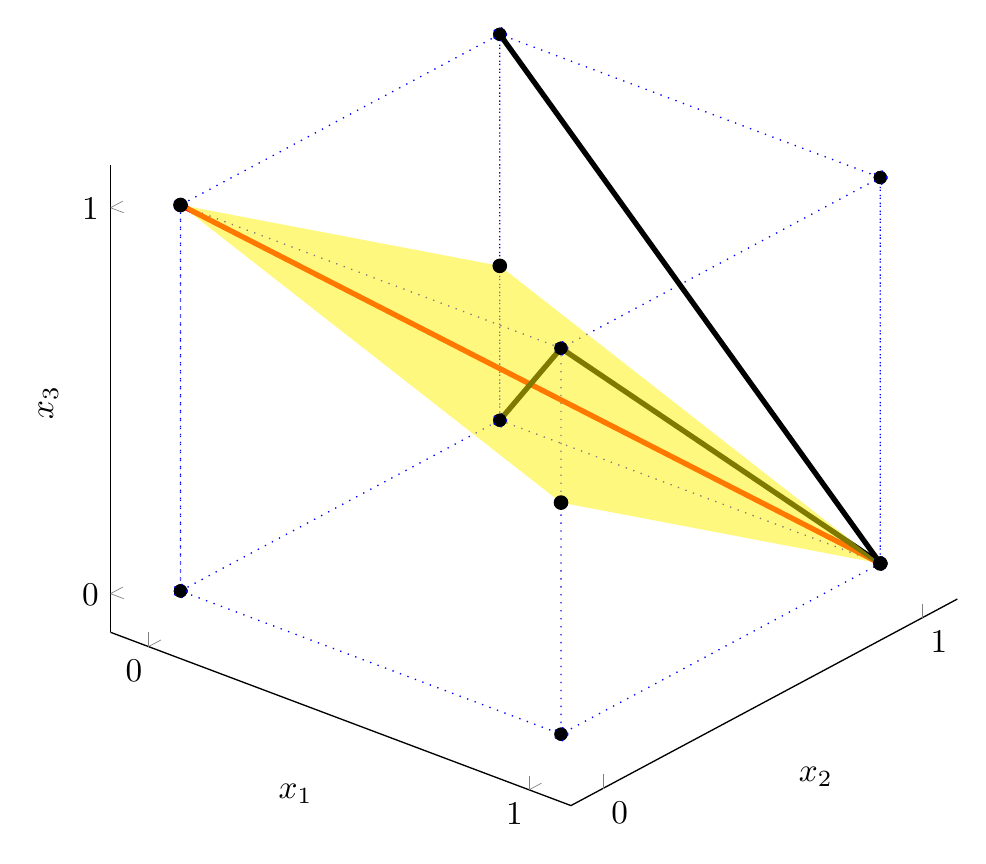
\begin{tikzpicture}[scale=1.2, x={({1}, {0})}]
    \begin{axis}[
      view/h=40,
      width=300pt,
      height=300pt,
      axis lines*=left,
      xmin=-0.1,xmax=1,
      ymin=-0.1,ymax=1,
      zmin=-0.1,zmax=1,
      enlargelimits=upper,
      xtick={0,1},
      ytick={0,1},
      ztick={0,1},
      xlabel={$x_1$},
      ylabel={$x_2$},
      zlabel={$x_3$}
    ]
      % pre-cube
      \addplot3[draw = blue, dotted, mark=*] coordinates {(0,0,0) (0,1,0) (0,1,1) (0,0,1) (0,0,0)
        (0,0,1) (1,0,1) (1,0,0) (0,0,0) (1, 0, 0) (1,1,0) (0,1,0) (0,1,1) (1,1,1) (1,1,0) (1,1,1) (1,0,1)};
      \addplot3[draw=red, ultra thick] coordinates {(0,0,1) (1,1,0)};
      \addplot3[fill=black, ultra thick] coordinates {(0,1,1) (1,1,0)};
      \addplot3[fill=black, ultra thick] coordinates {(1,0,1) (1,1,0)};
      \addplot3[fill=black, ultra thick] coordinates {(0,1,0) (1,0,1)};
      % upper
      \addplot3[draw = none, fill=yellow,fill opacity=0.5] coordinates {(1,0,3/5) (1,1,0) (0,1,2/5) (0,0,1) (1,0,3/5)};
      \addplot3 [only marks,mark=*] coordinates {(1,0,3/5) (1,1,0) (0,1,2/5) (0,0,1)};
      %\addplot3[mark=none,ultra thick] coordinates {(0,1,0) (1,1,0) (1,0,0) (1,0,1) (0,0,1)};
    \end{axis}
  \end{tikzpicture}
  \caption{Geometric visualisation of a given instance of the $3$-move SUBSET RECONFIGURATION problem.}
  \label{fig:geo_2}
\end{figure}


\begin{figure}[H]
  \centering
  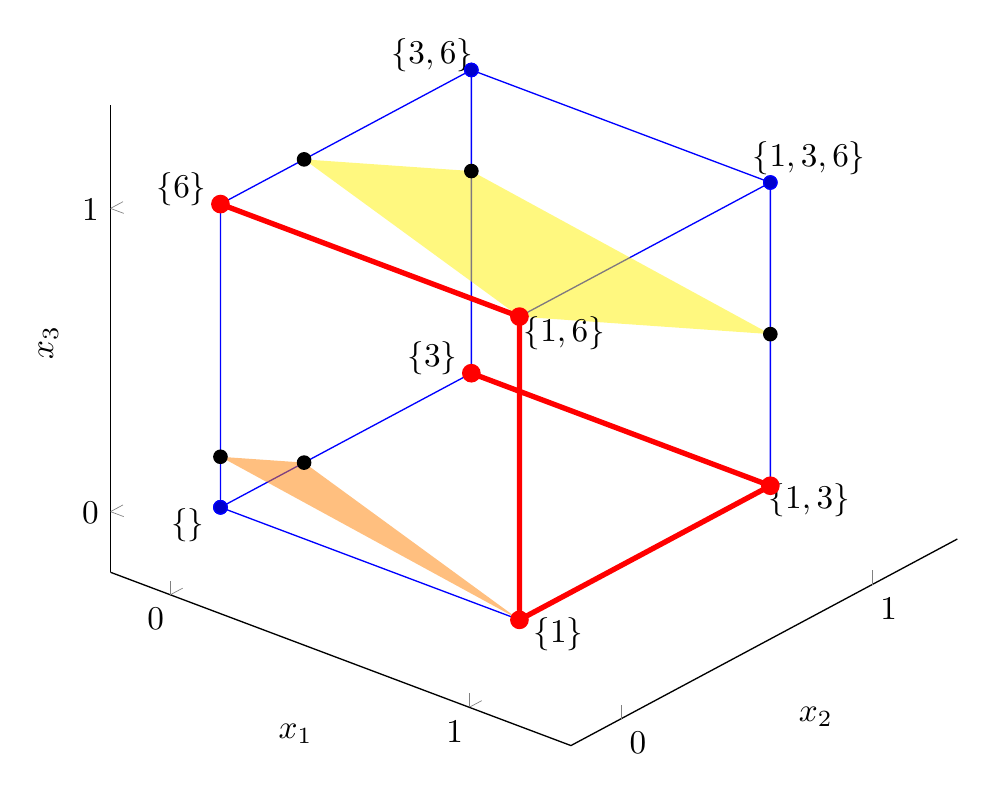
\begin{tikzpicture}[scale=1.2, x={({1}, {0})}]
    \begin{axis}[
      view/h=40,
      width=300pt,
      height=300pt,
      axis lines*=left,
      xmin=-0.2,xmax=1.2,
      ymin=-0.2,ymax=1.2,
      zmin=-0.2,zmax=1.2,
      enlargelimits=upper,
      xtick={0,1},
      ytick={0,1},
      ztick={0,1},
      xlabel={$x_1$},
      ylabel={$x_2$},
      zlabel={$x_3$}
    ]
      % pre-cube
      \addplot3 coordinates {(0,0,0) (0,1,0) (0,1,1) (0,0,1) (0,0,0)
        (0,0,1) (1,0,1) (1,0,0) (0,0,0) (1, 0, 0) (1,1,0) (0,1,0) (0,1,1) (1,1,1) (1,1,0) (1,1,1) (1,0,1)};
      % upper
      \addplot3[draw = none, fill=yellow,fill opacity=0.5] coordinates {(0,1,4/6) (1,1,1/2) (1,0,1)  (0,1/3,1) (0,1,4/6)};
      \addplot3 [only marks,mark=*] coordinates { (0,1,4/6) (1,1,1/2) (0,1/3,1)};

      %lower
      \addplot3[draw = none, fill=orange,fill opacity=0.5] coordinates {(1,0,0) (0,1/3,0) (0,0,1/6) (1,0,0)} ;
      \addplot3 [only marks,mark=*] coordinates { (1,0,0) (0,1/3,0) (0,0,1/6)};

      % solution paths
      \addplot3[draw=red, mark=none,ultra thick] coordinates {((0,0,1) (1,0,1) (1,0,0) (1,1,0) (0,1,0)};

      % initial and target confguration
      \addplot3 [only marks, mark=*, fill=red, draw=red, ultra thick] coordinates {(0,0,1) (1,0,1) (1,0,0) (1,1,0) (0,1,0)};

      \node (A) at (axis cs:0,-0.13,0) {$\{\}$};
      \node (B) at (axis cs:-0.13,1,0) {$\{3\}$};
      \node (C) at (axis cs:-0.13,1,1) {$\{3,6\}$};
      \node (D) at (axis cs:-0.13,0,1) {$\{6\}$};
      \node (E) at (axis cs:1.15,0,1) {$\{1,6\}$};
      \node (F) at (axis cs:1.13,0,0) {$\{1\}$};
      \node (G) at (axis cs:1.13,1,0) {$\{1,3\}$};
      \node (H) at (axis cs:1.13,1,1.13) {$\{1,3,6\}$};
    \end{axis}
  \end{tikzpicture}
  \caption{Geometric visualisation of a given knapsack reconfiguration problem.}
  \label{fig:geo_1}
\end{figure}



\begin{figure}[H]
  \centering
  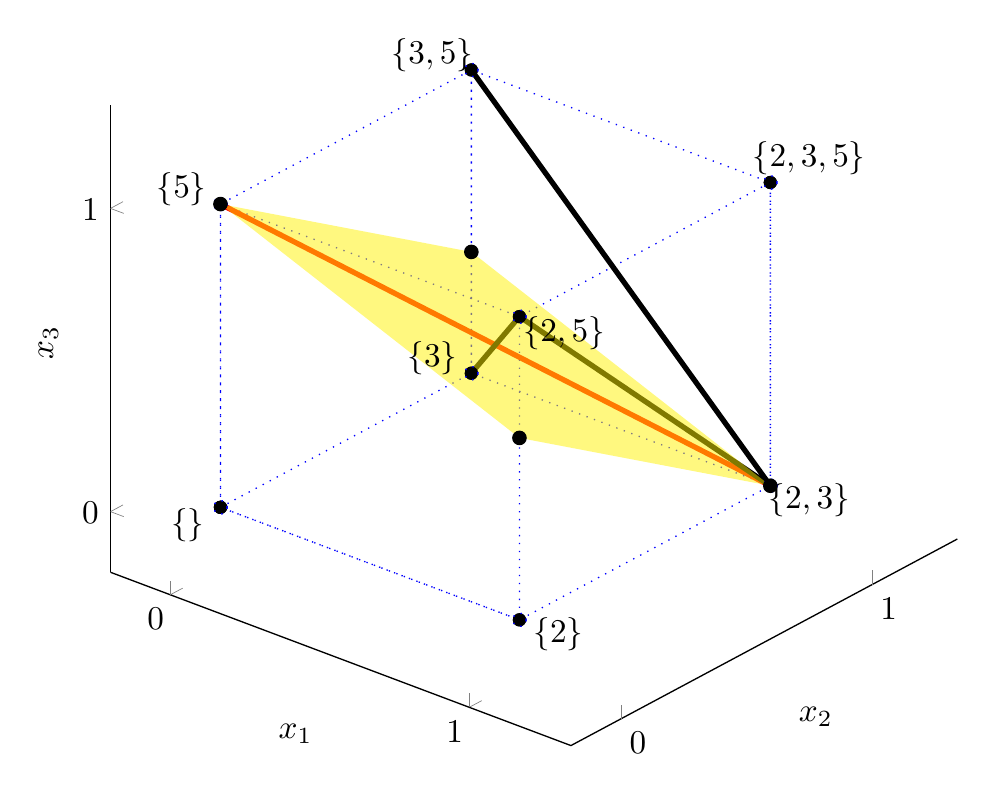
\begin{tikzpicture}[scale=1.2, x={({1}, {0})}]
    \begin{axis}[
      view/h=40,
      width=300pt,
      height=300pt,
      axis lines*=left,
      xmin=-0.2,xmax=1.2,
      ymin=-0.2,ymax=1.2,
      zmin=-0.2,zmax=1.2,
      enlargelimits=upper,
      xtick={0,1},
      ytick={0,1},
      ztick={0,1},
      xlabel={$x_1$},
      ylabel={$x_2$},
      zlabel={$x_3$}
    ]
      % pre-cube
      \addplot3[draw = blue, dotted, mark=*] coordinates {(0,0,0) (0,1,0) (0,1,1) (0,0,1) (0,0,0)
        (0,0,1) (1,0,1) (1,0,0) (0,0,0) (1, 0, 0) (1,1,0) (0,1,0) (0,1,1) (1,1,1) (1,1,0) (1,1,1) (1,0,1)};
      \addplot3[draw=red, ultra thick] coordinates {(0,0,1) (1,1,0)};
      \addplot3[fill=black, ultra thick] coordinates {(0,1,1) (1,1,0)};
      \addplot3[fill=black, ultra thick] coordinates {(1,0,1) (1,1,0)};
      \addplot3[fill=black, ultra thick] coordinates {(0,1,0) (1,0,1)};
      % upper
      \addplot3[draw = none, fill=yellow,fill opacity=0.5] coordinates {(1,0,3/5) (1,1,0) (0,1,2/5) (0,0,1) (1,0,3/5)};
      \addplot3 [only marks,mark=*] coordinates {(1,0,3/5) (1,1,0) (0,1,2/5) (0,0,1)};
      %\addplot3[mark=none,ultra thick] coordinates {(0,1,0) (1,1,0) (1,0,0) (1,0,1) (0,0,1)};

      \node (A) at (axis cs:0,-0.13,0) {$\{\}$};
      \node (B) at (axis cs:-0.13,1,0) {$\{3\}$};
      \node (C) at (axis cs:-0.13,1,1) {$\{3,5\}$};
      \node (D) at (axis cs:-0.13,0,1) {$\{5\}$};
      \node (E) at (axis cs:1.15,0,1) {$\{2,5\}$};
      \node (F) at (axis cs:1.13,0,0) {$\{2\}$};
      \node (G) at (axis cs:1.13,1,0) {$\{2,3\}$};
      \node (H) at (axis cs:1.13,1,1.13) {$\{2,3,5\}$};

    \end{axis}
  \end{tikzpicture}
  \caption{Geometric visualisation of a given instance of the $3$-move SUBSET RECONFIGURATION problem.}
  \label{fig:geo_2}
\end{figure}


\begin{figure}[H]
  \begin{center}
        \begin{tikzpicture}[scale=1]
          \node (1) at (0,0) [draw, dotted, rectangle, align=center] {$\mathcal{S} = \{2, 3, 4, 5, 7\}, x = 12$};
          \node (2)  [below=of 1, draw, rectangle, align=center] {$A_1 = \{2, 3, 7\}$};
          \node (3)  [below=of 2, draw, rectangle, align=center] {$\{5, 7\}$};
          \node (4) [below=of 3, draw, rectangle, align=center] {$A_2 = \{5, 3, 4\}$};

          \draw[->]  (2) to node [auto] {swap $2, 3$ with $5$} (3);
          \draw[->]  (3) to node [auto] {swap $7$ with $3,4$} (4);
        \end{tikzpicture}
  \end{center}
  \caption{$\PSPACE$-complete problems encountered and their relationship.}\label{fig:conclusion}
\end{figure}


\begin{figure}[H]
  \begin{center}
        \begin{tikzpicture}[scale=1]
          \node (1) at (0,0) [draw, dotted, rectangle, align=center] {$\mathcal{S} = \{2, 3, 4, 5, 7\}, l = 10$ and $u = 14$};
          \node (2)  [below=of 1, draw, rectangle, align=center] {$A_1 = \{2, 3, 7\}$};
          \node (3)  [below=of 2, draw, rectangle, align=center] {$\{3, 7\}$};
          \node (4) [below=of 3, draw, rectangle, align=center] {$A_2 = \{3, 4, 7\}$};

          \draw[->]  (2) to node [auto] {remove $2$} (3);
          \draw[->]  (3) to node [auto] {add $4$} (4);
        \end{tikzpicture}
  \end{center}
  \caption{$\PSPACE$-complete problems encountered and their relationship.}\label{fig:conclusion}
\end{figure}



\begin{figure}[H]
  \centering
  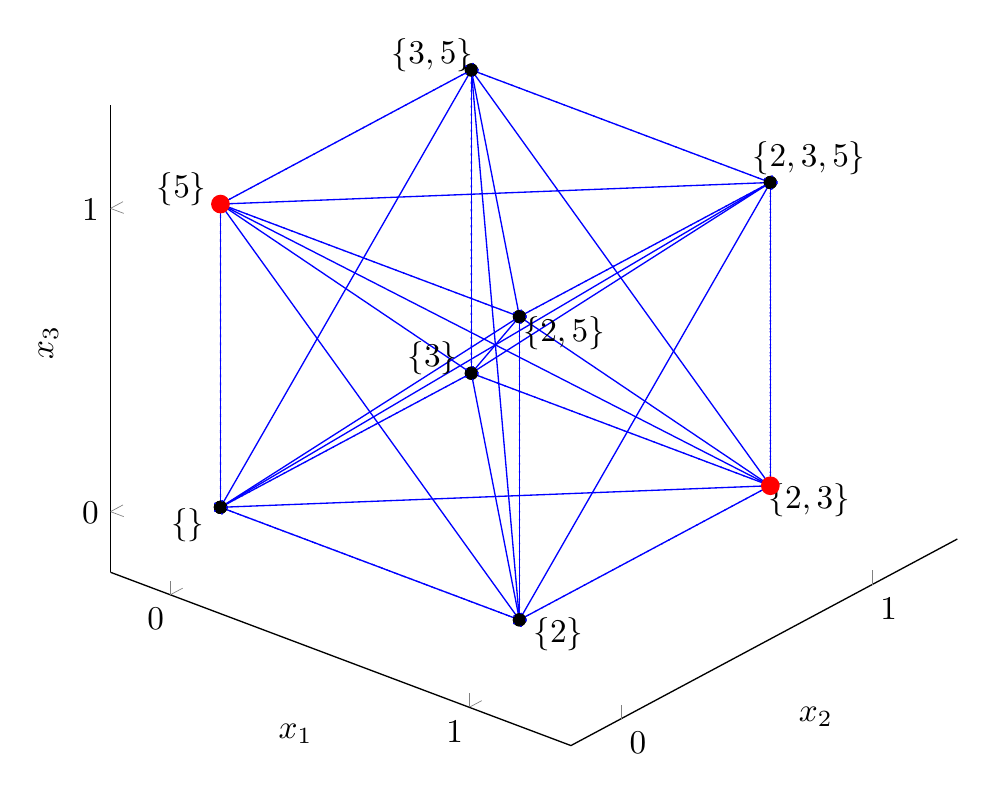
\begin{tikzpicture}[scale=1.2, x={({1}, {0})}]
    \begin{axis}[
      view/h=40,
      width=300pt,
      height=300pt,
      axis lines*=left,
      xmin=-0.2,xmax=1.2,
      ymin=-0.2,ymax=1.2,
      zmin=-0.2,zmax=1.2,
      enlargelimits=upper,
      xtick={0,1},
      ytick={0,1},
      ztick={0,1},
      xlabel={$x_1$},
      ylabel={$x_2$},
      zlabel={$x_3$}
    ]
      % pre-cube
      \addplot3[draw = blue, dotted, mark=*] coordinates {(0,0,0) (0,1,0) (0,1,1) (0,0,1) (0,0,0)
        (0,0,1) (1,0,1) (1,0,0) (0,0,0) (1, 0, 0) (1,1,0) (0,1,0) (0,1,1) (1,1,1) (1,1,0) (1,1,1) (1,0,1)};


      % initial and target confguration
      \addplot3 [only marks, mark=*, fill=red, draw=red, ultra thick] coordinates {(0,0,1) (1,1,0)};

      \addplot3[draw=blue] coordinates {(0,0,0) (0,1,0)};
      \addplot3[draw=blue] coordinates {(0,0,0) (0,1,1)};
      \addplot3[draw=blue] coordinates {(0,0,0) (0,0,1)};
      \addplot3[draw=blue] coordinates {(0,0,0) (1,0,1)};
      \addplot3[draw=blue] coordinates {(0,0,0) (1,0,0)};
      \addplot3[draw=blue] coordinates {(0,0,0) (1,1,0)};
      \addplot3[draw=blue] coordinates {(0,0,0) (1,1,1)};

      \addplot3[draw=blue] coordinates {(0,1,0) (0,1,1)};
      \addplot3[draw=blue] coordinates {(0,1,0) (0,0,1)};
      \addplot3[draw=blue] coordinates {(0,1,0) (1,0,1)};
      \addplot3[draw=blue] coordinates {(0,1,0) (1,0,0)};
      \addplot3[draw=blue] coordinates {(0,1,0) (1,1,0)};
      \addplot3[draw=blue] coordinates {(0,1,0) (1,1,1)};

      \addplot3[draw=blue] coordinates {(0,1,1) (0,0,1)};
      \addplot3[draw=blue] coordinates {(0,1,1) (1,0,1)};
      \addplot3[draw=blue] coordinates {(0,1,1) (1,0,0)};
      \addplot3[draw=blue] coordinates {(0,1,1) (1,1,0)};
      \addplot3[draw=blue] coordinates {(0,1,1) (1,1,1)};


      \addplot3[draw=blue] coordinates {(0,0,1) (1,0,0)};
      \addplot3[draw=blue] coordinates {(0,0,1) (1,1,0)};
      \addplot3[draw=blue] coordinates {(0,0,1) (1,1,1)};

      \addplot3[draw=blue] coordinates {(1,0,1) (0,0,1)};
      \addplot3[draw=blue] coordinates {(1,0,1) (1,0,0)};
      \addplot3[draw=blue] coordinates {(1,0,1) (1,1,0)};
      \addplot3[draw=blue] coordinates {(1,0,1) (1,1,1)};

      \addplot3[draw=blue] coordinates {(1,0,0) (1,1,0)};
      \addplot3[draw=blue] coordinates {(1,0,0) (1,1,1)};

      \addplot3[draw=blue] coordinates {(1,1,0) (1,1,1)};



      \node (A) at (axis cs:0,-0.13,0) {$\{\}$};        % 000
      \node (B) at (axis cs:-0.13,1,0) {$\{3\}$};       % 010
      \node (C) at (axis cs:-0.13,1,1) {$\{3,5\}$};     % 011
      \node (D) at (axis cs:-0.13,0,1) {$\{5\}$};       % 001
      \node (E) at (axis cs:1.15,0,1) {$\{2,5\}$};      % 101
      \node (F) at (axis cs:1.13,0,0) {$\{2\}$};        % 100
      \node (G) at (axis cs:1.13,1,0) {$\{2,3\}$};      % 110
      \node (H) at (axis cs:1.13,1,1.13) {$\{2,3,5\}$}; % 111

    \end{axis}
  \end{tikzpicture}
  \caption{Geometric visualisation of a given instance of the $3$-move SUBSET RECONFIGURATION problem.}
  \label{fig:geo_2}
\end{figure}


\begin{figure}[H]
  \centering
  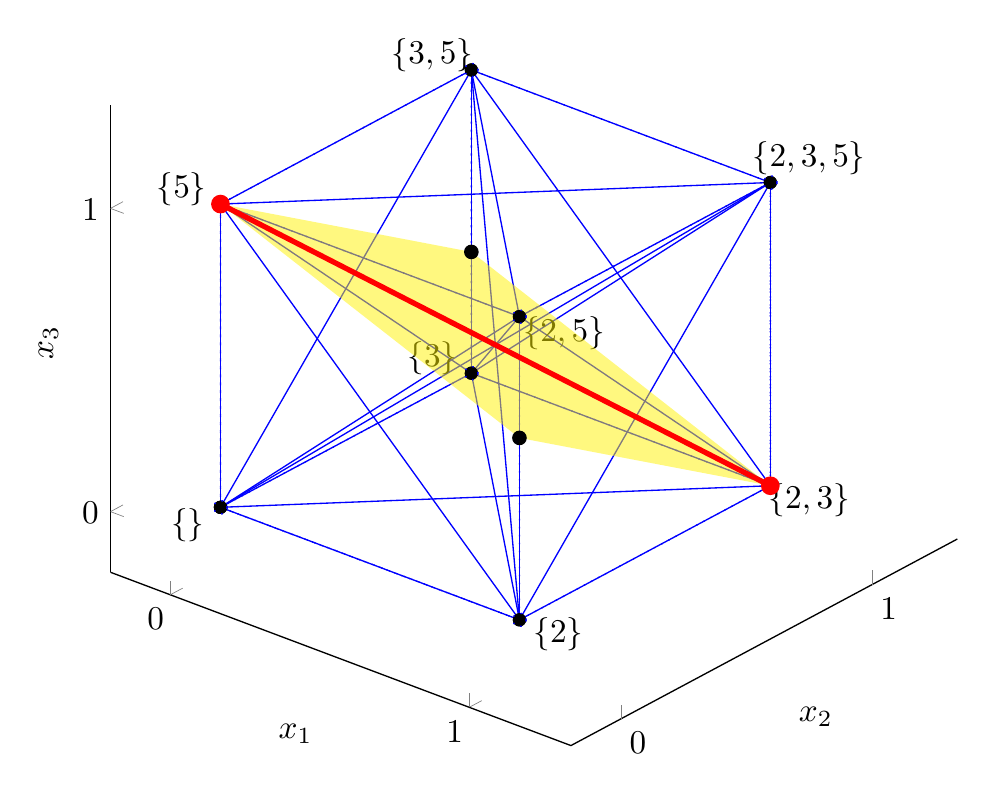
\begin{tikzpicture}[scale=1.2, x={({1}, {0})}]
    \begin{axis}[
      view/h=40,
      width=300pt,
      height=300pt,
      axis lines*=left,
      xmin=-0.2,xmax=1.2,
      ymin=-0.2,ymax=1.2,
      zmin=-0.2,zmax=1.2,
      enlargelimits=upper,
      xtick={0,1},
      ytick={0,1},
      ztick={0,1},
      xlabel={$x_1$},
      ylabel={$x_2$},
      zlabel={$x_3$}
    ]
      % pre-cube
      \addplot3[draw = blue, dotted, mark=*] coordinates {(0,0,0) (0,1,0) (0,1,1) (0,0,1) (0,0,0)
        (0,0,1) (1,0,1) (1,0,0) (0,0,0) (1, 0, 0) (1,1,0) (0,1,0) (0,1,1) (1,1,1) (1,1,0) (1,1,1) (1,0,1)};

      \addplot3[draw=blue] coordinates {(0,0,0) (0,1,0)};
      \addplot3[draw=blue] coordinates {(0,0,0) (0,1,1)};
      \addplot3[draw=blue] coordinates {(0,0,0) (0,0,1)};
      \addplot3[draw=blue] coordinates {(0,0,0) (1,0,1)};
      \addplot3[draw=blue] coordinates {(0,0,0) (1,0,0)};
      \addplot3[draw=blue] coordinates {(0,0,0) (1,1,0)};
      \addplot3[draw=blue] coordinates {(0,0,0) (1,1,1)};

      \addplot3[draw=blue] coordinates {(0,1,0) (0,1,1)};
      \addplot3[draw=blue] coordinates {(0,1,0) (0,0,1)};
      \addplot3[draw=blue] coordinates {(0,1,0) (1,0,1)};
      \addplot3[draw=blue] coordinates {(0,1,0) (1,0,0)};
      \addplot3[draw=blue] coordinates {(0,1,0) (1,1,0)};
      \addplot3[draw=blue] coordinates {(0,1,0) (1,1,1)};

      \addplot3[draw=blue] coordinates {(0,1,1) (0,0,1)};
      \addplot3[draw=blue] coordinates {(0,1,1) (1,0,1)};
      \addplot3[draw=blue] coordinates {(0,1,1) (1,0,0)};
      \addplot3[draw=blue] coordinates {(0,1,1) (1,1,0)};
      \addplot3[draw=blue] coordinates {(0,1,1) (1,1,1)};


      \addplot3[draw=blue] coordinates {(0,0,1) (1,0,0)};
      \addplot3[draw=blue] coordinates {(0,0,1) (1,1,0)};
      \addplot3[draw=blue] coordinates {(0,0,1) (1,1,1)};

      \addplot3[draw=blue] coordinates {(1,0,1) (0,0,1)};
      \addplot3[draw=blue] coordinates {(1,0,1) (1,0,0)};
      \addplot3[draw=blue] coordinates {(1,0,1) (1,1,0)};
      \addplot3[draw=blue] coordinates {(1,0,1) (1,1,1)};

      \addplot3[draw=blue] coordinates {(1,0,0) (1,1,0)};
      \addplot3[draw=blue] coordinates {(1,0,0) (1,1,1)};

      \addplot3[draw=blue] coordinates {(1,1,0) (1,1,1)};

      \node (A) at (axis cs:0,-0.13,0) {$\{\}$};        % 000
      \node (B) at (axis cs:-0.13,1,0) {$\{3\}$};       % 010
      \node (C) at (axis cs:-0.13,1,1) {$\{3,5\}$};     % 011
      \node (D) at (axis cs:-0.13,0,1) {$\{5\}$};       % 001
      \node (E) at (axis cs:1.15,0,1) {$\{2,5\}$};      % 101
      \node (F) at (axis cs:1.13,0,0) {$\{2\}$};        % 100
      \node (G) at (axis cs:1.13,1,0) {$\{2,3\}$};      % 110
      \node (H) at (axis cs:1.13,1,1.13) {$\{2,3,5\}$}; % 111

      % upper
      \addplot3[draw = none, fill=yellow,fill opacity=0.5] coordinates {(1,0,3/5) (1,1,0) (0,1,2/5) (0,0,1) (1,0,3/5)};
      \addplot3 [only marks,mark=*] coordinates {(1,0,3/5) (1,1,0) (0,1,2/5) (0,0,1)};

      \addplot3[draw=red, ultra thick, mark=none] coordinates {(0,0,1) (1,1,0)};

      % initial and target confguration
      \addplot3 [only marks, mark=*, fill=red, draw=red, ultra thick] coordinates {(0,0,1) (1,1,0)};

    \end{axis}
  \end{tikzpicture}
  \caption{Geometric visualisation of a given instance of the $3$-move SUBSET RECONFIGURATION problem.}
  \label{fig:geo_2}
\end{figure}
